\documentclass[10pt]{article}
\usepackage{icmlko}

\icmlmeta{IP 파운데이션 월드모델}{268}{같은 줄을 세운다}{코호트를 판정 기준으로 바꿔도 순위가 한 자리도 안 바뀐다 --- 그리고 섞음의 한쪽이 죽었다}

\begin{document}

\twocolumn[
\icmlheader

\begin{abstract}
노트 267이 코호트 통제를 \emph{진단}으로 썼다 --- 달력 기준선은 41\%
무너지고 모형은 1\%만 준다. 그러면 \textbf{판정 기준을 아예 코호트 안
$\rho$ 로 바꾸면 어떤가.} 배포에서 예측할 작품들은 다 비슷한 시기에 나오므로
코호트 안 $\rho$ 가 실제 쓰임에 더 가깝다는 논리가 선다. 주요 정식화 다섯을
두 눈금으로 줄 세웠다. \textbf{한 자리도 안 바뀐다} --- spearman $=+1.000$.
코호트 통제는 모두를 조금씩 내릴 뿐이고(F18 $-$0.0036 · F23 $-$0.0106 ·
F21 $-$0.0117 · F9 $-$0.0140) 그 크기가 순위를 못 뒤집는다. \textbf{판
$\rho$ 를 계속 쓴다} --- 코호트는 진단으로 남긴다. 재면서 딴 것을 봤다.
\textbf{F18 배깅나무(0.4845)가 F23 섞음(0.4839)을 앞선다.} 짝지어 재니
$-$0.0010 ($t{=}-0.17$)로 \textbf{1 SE 안 동점}이고, F18 대 F21 은
$-$0.0300($t{=}-2.82$)로 \textbf{유의}하다. F23 은 정의상 F21 과 F18 을
반씩 순위 평균한 것이므로 --- \textbf{섞이는 한쪽이 유의하게 나쁘고 섞음이
나은 쪽과 동점이면 그 섞음은 할 일이 없다.} 노트 126의 동점 규칙(1 SE 안이면
좁은 쪽)대로 \textbf{챔피언이 F23 에서 F18 로 돌아간다.} 노트 215가 공휴일을
채우고 F18 $\to$ F21 을 옮겼고, 노트 224 이후 F23 이 챔피언이었다. 이번이
네 번째 이동이고, 네 번 다 \textbf{자료나 하네스를 고친 뒤}에 일어났다 ---
정식화를 새로 만들어서가 아니다.
\end{abstract}
]

\section{판정 기준을 바꿔 볼 만한 이유}

노트 267은 코호트 통제를 진단으로 썼다. 그런데 논리를 한 걸음 밀면 판정
기준을 바꿀 이유가 된다.

\begin{quote}\small
배포에서 예측할 것은 \emph{아직 안 나온} 작품들이고, 그것들은 다 비슷한
시기에 나온다. 그러면 ``서로 다른 시기의 작품을 한 줄로 세우는'' 능력은
쓸모가 없고, \textbf{같은 시기 안에서 세우는} 능력만 쓸모가 있다.
\end{quote}

지금 판 $\rho$ 는 유보 2,565건을 통째로 한 줄로 세운다. 그 안에 2025년부터
2027년까지가 섞여 있고, 노트 267이 쟀듯 그 시간 축만으로도 0.2287 이 나온다.

\section{한 자리도 안 바뀐다}

주요 정식화 다섯을 두 눈금으로 줄 세웠다.

\begin{figure}[t]
\centering

\includegraphics[width=\columnwidth]{figs/rank.pdf}
\caption{왼쪽 --- 두 눈금. 오른쪽 --- 순위를 이은 선.}
\end{figure}

\begin{center}\small
\begin{tabular}{lrrrr}
\hline
정식화 & 판 $\rho$ & 코호트 $\rho$ & 차 & 순위 \\
\hline
F18 배깅나무 & 0.4845 & 0.4809 & $-$0.0036 & 1 $\to$ 1 \\
F23 섞음 & 0.4839 & 0.4733 & $-$0.0106 & 2 $\to$ 2 \\
F21 능형 & 0.4542 & 0.4425 & $-$0.0117 & 3 $\to$ 3 \\
F9 순위가능도 & 0.4468 & 0.4328 & $-$0.0140 & 4 $\to$ 4 \\
F1 프로크루스테스 & 0.2147 & 0.2142 & $-$0.0005 & 5 $\to$ 5 \\
\hline
\end{tabular}
\end{center}

\[ \text{spearman}(\text{판}, \text{코호트}) = +1.000. \]

\textbf{선이 하나도 안 엇갈린다.} 코호트 통제는 모두를 조금씩 내리는데
($-$0.004 $\sim$ $-$0.014) 그 폭이 정식화 사이 간격보다 작다.

그래서 \textbf{판 $\rho$ 를 계속 쓴다.} 눈금을 바꾸는 것은 공짜가 아니다 ---
코호트 안 $\rho$ 는 도메인마다 반년 조각이 몇 개냐에 따라 표본이 갈리고
(팝업 · 펀딩은 조각이 하나라 아예 못 낸다) 해석이 어렵다. \textbf{순위를
못 바꾸는 눈금으로 갈아탈 이유가 없다.} 코호트는 노트 267처럼 진단으로
남긴다.

\section{재다가 본 것 --- 섞음의 한쪽이 죽었다}

표 맨 위가 F23 이 아니다.

\begin{figure}[t]
\centering
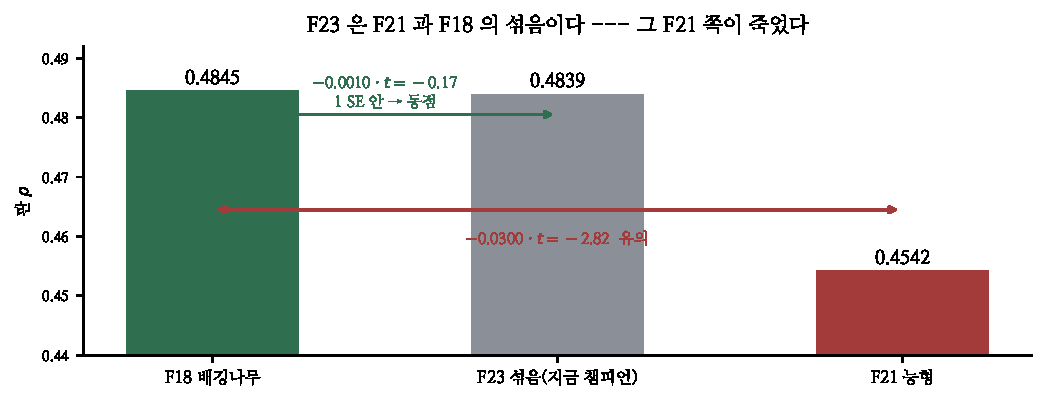
\includegraphics[width=\columnwidth]{figs/champ.pdf}
\caption{F23 은 F21 과 F18 을 반씩 순위 평균한 것이다.}
\end{figure}

\begin{center}\small
\begin{tabular}{lrrl}
\hline
견줌 & 차 & $t$ & 판정 \\
\hline
F18 $\to$ F23 & $-$0.0010 & $-$0.17 & \textbf{1 SE 안 동점} \\
F18 $\to$ F21 & $-$0.0300 & $-$2.82 & 유의 \\
F21 $\to$ F23 & $+$0.0296 & $+$5.23 & 유의 \\
\hline
\end{tabular}
\end{center}

F23 은 정의상 $0.5 \cdot \text{rank}(\text{F21}) + 0.5 \cdot
\text{rank}(\text{F18})$ 이다. 지금 상태는

\begin{itemize}
\item 섞이는 한쪽(F21)이 다른 쪽(F18)보다 \textbf{유의하게 나쁘고}
\item 섞음(F23)이 나은 쪽(F18)과 \textbf{동점}이다.
\end{itemize}

\textbf{그러면 그 섞음은 할 일이 없다.} 노트 126의 동점 규칙 --- 짝지은
1 SE 안이면 좁은 쪽 --- 대로 \textbf{챔피언이 F18 로 돌아간다.}

도메인별로 보면 섞음이 무엇을 하고 있었는지 보인다.

\begin{center}\small
\begin{tabular}{lrrrr}
\hline
 & 웹툰 & 애니 & 모바일 & 게임 \\
\hline
F18 & \textbf{0.453} & 0.505 & \textbf{0.535} & 0.622 \\
F23 & 0.441 & \textbf{0.538} & 0.524 & \textbf{0.634} \\
F21 & 0.403 & 0.504 & 0.507 & 0.618 \\
\hline
\end{tabular}
\end{center}

섞음은 애니($+$0.033)와 게임($+$0.012)을 올리고 웹툰($-$0.012)과
모바일($-$0.011)을 내린다. 몫이 큰 웹툰이 내려가서 판에서 상쇄된다 ---
노트 247이 만든 눈금으로 읽으면 자리바꿈이다.

\section{네 번째 이동, 네 번 다 같은 이유}

챔피언이 옮겨 간 자리를 모아 보면 무늬가 있다.

\begin{center}\small
\begin{tabular}{lll}
\hline
노트 & 이동 & 계기 \\
\hline
215 & F18 $\to$ F21 & 공휴일 목록을 채웠다 \\
224 & F21 $\to$ F23 & 라벨 두 종류를 갈랐다 \\
233 & (판정치 고침) & NaN 전파를 고쳤다 \\
\textbf{268} & \textbf{F23 $\to$ F18} & \textbf{새는 축 둘을 막았다} \\
\hline
\end{tabular}
\end{center}

\textbf{네 번 다 정식화를 새로 만들어서가 아니라 자료나 하네스를 고친 뒤에
일어났다.} 이 실험실이 노트 125에서 ``정식화 포트폴리오''로 돌아섰는데,
정작 순위를 바꾼 것은 언제나 \emph{아래층}이었다.

\paragraph{남은 것}
\begin{center}\small
\begin{tabular}{ll}
\hline
갈래 & 왜 \\
\hline
F23 을 지울까 & 두 부품 중 하나가 죽었다. 다른 가중은? \\
F18 이 왜 이겼나 & 새는 축을 막으니 나무가 살아났다 \\
도서 & 다섯 번째 --- 아직 안 팠다 \\
\texttt{SOURCE} & 34/45 쌍 \\
\hline
\end{tabular}
\end{center}

\paragraph{규약} 판정 눈금을 바꾸자는 제안이 나오면 \textbf{먼저 두 눈금으로
줄을 세워 본다.} 순위가 같으면 안 바꾼다 --- 새 눈금이 더 옳아 보여도,
바꾸는 값이 0 이면 해석만 어려워진다.

\end{document}
